\chapter{Исследование источника когерентного излучения на основе оптической инжекции на устойчивость к лазерному засеиванию мощным излучением}\label{ch:ch5}
\renewcommand{\thefigure}{5.\arabic{figure}} % Plain numbering
\setcounter{figure}{0}                     % Reset if needed
\renewcommand{\thetable}{5.\arabic{table}}
\setcounter{table}{0} 
\section{Введение}\label{ch:ch5/sect1}
На данный момент в практических системах квантового распределения ключей в качестве источника одиночных фотонов используется ослабленный лазерный источник. Это открывает для злоумышленника множество возможностей атаковать источник КРК и получить информацию о секретном ключе. Обычно в качестве контрмеры против атак на источник света КРК рекомендуется использовать некоторую степень изоляции. Однако практические оптические компоненты также могут изменять значение изоляции при внешнем воздействии или под влиянием условий окружающей среды. В данной работе продемонстрировано, что источник лазерного излучения на основе лазерной инжекции обладает очень высокой устойчивостью к атакам внешним засевом, и рекомендуется использовать эту схему в качестве безопасного источника фотонов для систем КРК.
Квантовое распределение ключей (КРК) позволяет двум сторонам распределять секретный ключ по ненадежному каналу, используя квантово-механические свойства одиночных фотонов. Протоколы КРК в принципе не поддаются взлому. Однако их практическая реализация демонстрирует длинный список побочных каналов, которые могут предоставить подслушивающему лицу дополнительную информацию о секретном ключе и сделать систему, использующую его, небезопасной~\cite{sun2022, makarov2023}. Такие побочные каналы почти всегда являются результатом отличия аппаратного обеспечения от его идеальной модели. 

Одним из наиболее ярких примеров несовершенных устройств являются практические источники фотонов. На сегодняшний день в практических системах КРК используются сильно ослабленные лазерные импульсы от полупроводниковых лазерных диодов (ЛД), а не истинные однофотонные источники, поскольку последние пока не позволяют достичь практической скорости передачи ключей ~\cite{zahidy2024}.
Однако, поскольку полупроводниковые лазеры очень чувствительны ко внешним воздействиям, существует несколько атак с лазерным засевом, которые открывают лазейки для подслушивающих~\cite{huang2019, pang2020, lovic2023}. Например, предыдущие экспериментальные исследования показали, что мощности инжекции в диапазоне 100 - 160 нВт может быть достаточно для управления интенсивностью импульсов Алисы~\cite{huang2019, pang2020}, а мощности даже около 1 нВт может быть достаточно для частичного управления фазой импульсов Алисы~\cite{lovic2023}.

В этой работе обращается внимание на то, что описанные выше атаки с лазерным засевом относятся к источнику света, основанному на одном лазерном диоде с усилением. В то же время, ЛД источники с оптической инжекцией стали широко использоваться в квантовой криптографии, особенно в реализациях квантового распределения ключей с недоверенным приемным узлом (НПУ КРК)~\cite{wei2020,woodward2021}.

Схема с оптической инжекцией незаменима для приложений, требующих высокой видности интерференции между независимыми лазерными источниками. Техника инжекции света значительно улучшает интерференцию за счет низкого джиттера времени импульса и синхронизации частотных чирпов при сохранении случайности фазы излучаемых лазерных импульсов~\cite{comandar2016}. Более того, последние исследования показывают, что лазерный источник с оптической инжекцией позволяет уменьшить флуктуации интенсивности и тем самым увеличить безопасную скорость передачи ключей при реализации техники состояний-ловушек~\cite{xie2019}. %\AP{add ref}%
 
К сожалению, конфигурация источника с оптической фазовой синхронизацией ранее не тестировалась на устойчивость к атакам с засевом лазерным излучением. В этой работе впервые исследуем ее оптические характеристики при внешней лазерной атаке и проводим анализ защищенности при наличии изменений выходного сигнала. В работе показано, что конфигурация источника фотонов с оптической фазовой синхронизацией является эффективной контрмерой против известных атак на источник фотонов КРК. Между тем, это исследование демонстрирует и другие эффекты, которые могут иметь место только в исследуемой конфигурации источника. В частности, ведомый лазер действует как ненасыщенный оптический усилитель. Это приводит к независимому усилению сигналов ведущего и Евы и позволяет злоумышленнику извлечь дополнительную информацию о секретном ключе
\begin{figure*}
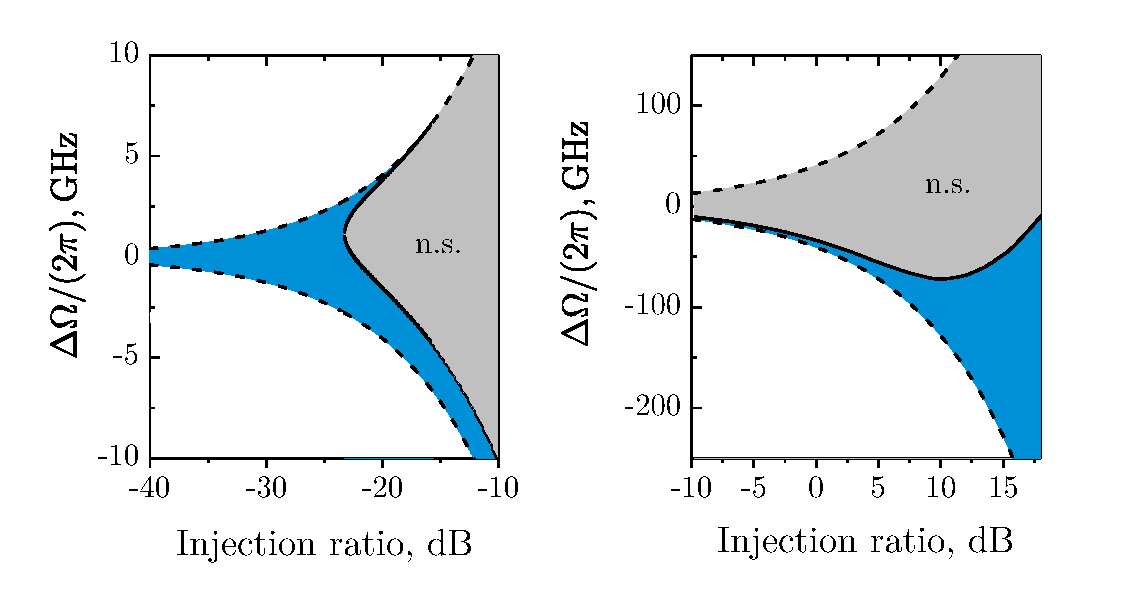
\includegraphics{images/StabilityDiagramsFreq.pdf}
\caption{Карта фазовой синхронизации двух лазеров(область стабильной синхронизации обозначена синим цветом).}
\label{fig:injection}
\end{figure*}
\section{Теоретическое описание метода оптической синхронизации}\label{ch:ch5/sect2}
\label{sec:theory}

\subsection{Полупроводниковые источники света с инжекционной синхронизацией}

Фазовая синхронизация с помощью оптической инжекции - это метод оптической частотной и фазовой синхронизации, основанный на освещении лазерного резонатора внешним светом. Источник с оптической инжекцией содержит "ведущий' лазер, который обеспечивает внешнее излучение для воздействия на 'ведомый' лазер~\cite{liu2020}. 

В зависимости от интенсивностей и спектральных показателей ведущего и ведомого ЛД, источник может обеспечивать режим свободной генерации, стабильной или нестабильной синхронизации~\cite{lau2008}. Эти режимы определяются как области диаграммы с коэффициентом инжекции и частотной подстройкой в виде координат, как показано на \cref{fig:injection}. Частота перестройки - это разность между частотами ведущего и свободно работающего ведомого каналов. Коэффициент инжекции $R_I$ определяется как 

\begin{equation}
\label{eq:injection_coeffitient}
	R_I = -10\times\lg\left({\frac{Q_c^M}{Q_c}} \right),
\end{equation}
%
где $Q_c^M$ и $Q_c$ значения интенсивности ведущего и ведомого лазеров в режиме свободной генерации в установившемся режиме, соответственно.
Отметим также, что в импульсном режиме работы ЛД интенсивности $Q_c^M$ и $Q_c$ определяются пиковыми мощностями импульсов как 
\begin{equation}
\label{eq:intens}
	Q = \frac{<P>}{f_R\times\tau_P},
\end{equation}
где $<P>$ - средняя мощность в Ваттах, $f_R$ - частота повторения импульсов, Гц, и $\tau_P$ - длительность импульса, с.
\begin{table}
	\centering
	\caption{Параметры лазера для создания оптической инжекции} 
	\label{tab:sim_param}
	\begin{tabular}[t]{@{\extracolsep{1.8ex}}l@{}c@{\quad}l@{}c@{}}
		\hline\hline
		Параметр		&Значение  			&Параметр 	& Значение	\\ 
		\hline
		$N_{th}$		&$5.5\times10^7$ 	&$N_{tr}$  		& $5.0\times10^7$		\\   
		$\tau_{e}$		&$1~ns$	&$\tau_{ph}$ 	&$1~ps$		\\ 
		$C_{sp}$		&$10^{-5}$ 		& $\Gamma$	& 0.12				\\
		$\alpha$		&5 				& $\kappa_{inj}$	& $5.0\times10^{10} ns^{-1}$	\\  
		I			&$22~mA$	& $\gamma_Q$	& 0				\\
		\hline\hline
	\end{tabular}
	\label{tab:all}
\end{table}
Когда источник работает в режиме стабильной синхронизации, ведомый лазер будет вынужден синхронизироваться с ведущим, то есть излучать на той же частоте. В целом, согласно карте синхронизации на рисунке \ref{fig:injection}, диапазон синхронизации частоты становится больше с увеличением коэффициента инжекции~\cite{wang2013}. Между тем, в реальных источниках света для систем КРК коэффициент инжекции отрицательный. Низкий коэффициент инжекции обусловлен двумя факторами. Во-первых, излучение ведущего не полностью заходит в резонатор ведомого. А второй фактор связан с длительностью импульса в соответствии с \ref{eq:intens}. Широко используемый случай реализации оптической схемы предполагает длительность импульса ведомого лазера в несколько раз меньше, чем у ведущего ЛД (в два раза и больше). Это позволяет избежать высокоамплитудных релаксационных осцилляций в выходных импульсах за счет засева ведомого лазера только частью импульса без частотного чирпа по интенсивности ведущего. В итоге, для получения высокой стабильности интенсивности исследуемых источников ведущий и свободно работающий ведомый ЛД должны иметь как можно более близкую рабочую длину волны.

%\subsection{Многоволновое усиление в полупроводниковых усиливающих средах}

%Традиционно полупроводниковые источники с оптической инжекцией включают в себя два лазера, ведущий и ведомый лазерные диоды, и теоретически они изучаются в рамках концепции этой конструкции. Однако в этом разделе мы также хотели бы рассмотреть это явление в аспекте усиления излучения в ведомом лазере. Это необходимо для понимания анализа экспериментальных результатов и атак на источник КРК с оптической инжекцией. Конструкции волноводов и материал усиления одинаковы или похожи для лазерных диодов и полупроводниковых оптических усилителей (ПОУ). Разница в том, что в лазерах для генерации и поддержания колебаний вокруг среды усиления формируется резонатор, и сигнал проходит несколько кругов внутри резонатора перед выходом~\cite{chen2022}. Поэтому предположим, что ведомый лазер - это двухпроходной ПОУ с неидеальным входом, который дает отражения
\subsection{Статистика интерференции фазово-рандомизированного классического света}

Статистические свойства интерференционного сигнала фазово-рандомизированного классического света хорошо изучены и имеют строгие модели, учитывающие все характеристики импульсов~\cite{shakhovoy2020, shakhovoy2021}. Недавно они были разработаны для реализации высококачественных квантовых генераторов случайных сигналов, основанных на интерференции фазово-рандомизированных импульсов. Благодаря этому, используя функцию плотности вероятности интерференционного сигнала, можно дать оценку видимости интерференции, объяснить влияние на нее свойств импульса и, наконец, что очень важно, настроить источник света так, чтобы получить наибольшую видимость интерференции. Поэтому в наших экспериментах мы не измеряем двухфотонную интерференцию, а измеряем и анализируем функцию плотности вероятности интерференции классического света. 

Процедура состоит в следующем. Она включает в себя реализацию несимметричного интерферометра с линией задержки, обеспечивающей время задержки, кратное периоду повторения импульсов. Это приводит к интерференции между импульсами, испускаемыми в разное время. Далее с помощью осциллографа накапливается большая выборка измерений площади интерференционного сигнала и строится гистограмма зависимости числа импульсов от их площади.

В работе~\cite{shakhovoy2021}, авторы показали, что колоколообразный лазерный импульс будет иметь двухпиковую форму ФПВ, где пики будут располагаться на интенсивности конструктивной и деструктивной интерференции, как показано на~\cref{fig:PDF}.
\begin{figure}
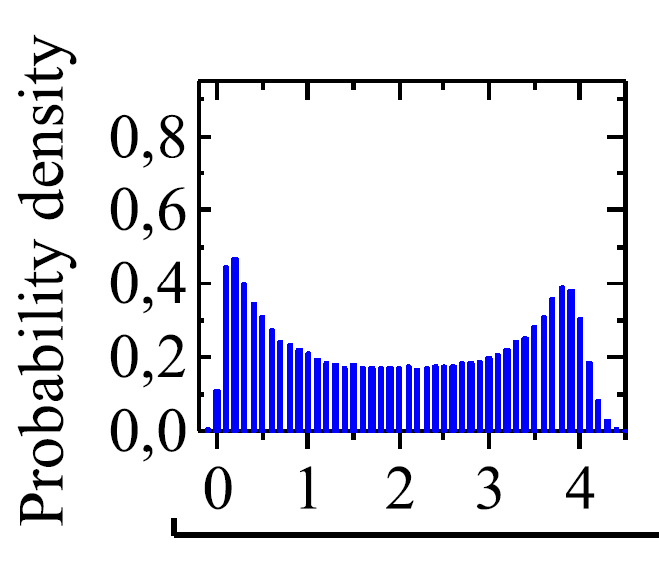
\includegraphics[width=\linewidth]{PDF}
\caption{Нормализованная функция плотности распределения интерференции колоколообразных импульсов без чирпа~\cite{shakhovoy2021}.}
\label{fig:PDF}
\end{figure}
Чтобы сравнить функции плотности вероятности (ФПВ) друг с другом, введем экспериментальную видимость интерференции
\begin{equation}
\label{eq:visibility}
	\eta = {\frac{S_{max} - S_{min}}{4\sqrt{s_1 s_2}}},
\end{equation}
где $S_{max}$ и $S_{min}$ - нормированные интенсивности конструктивной и деструктивной интерференции, определяемые по максимальным экспериментальным вероятностям, $s_1$ и $s_2$ - интенсивности начальных импульсов, которые принимаются равными 1.
\section{Проведение эксперимента}\label{ch:ch5/sect3}
\label{sec:experiment} 

На рисунке \Cref{fig:setup} показана экспериментальная установка. Она включает в себя три основные части. Это источник света Алисы, атакующий лазер злоумышленника и измерительное оборудование.
\begin{figure}
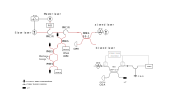
\includegraphics[width=\linewidth]{setup}
\caption{Экспериментальная установка (PM-волокна выделены красным цветом): VOA - перестраиваемый оптический аттенюатор, BS - светоделитель, PMCIR - циркулятор с сохранением поляризации, PMBS - светоделитель с сохранением поляризации, PG - генератор импульсов, OPM - измеритель оптической мощности, OSC - осциллограф, OSA - оптический анализатор спектра, BS - светоделитель, LT - световая ловушка, FM - зеркало Фарадея. Коэффициент связи светоделителя (BS) обозначается 99 =: 1× означает, что $99\%$ света проходит в порт, горизонтально противоположный графическому обозначению СД, в то время как $1\%$ света
свет попадает в другой порт}.
\label{fig:setup}
\end{figure}
\subsection{Источник света на испытаниях}

В этой работе реализован оптический источник излучения с оптической инжекцией. Его оптическая схема обозначена как Alice в \cref{fig:setup}. Ведущий лазер излучает импульсы со случайной фазой. Они поступают в ведомый лазер через волоконно-оптический циркулятор PMCIR1 (PMCIR-3-A-1550-900-5-08-FA, Optel) из порта~1 в порт~2 и ``засевают'' ведомый лазер. Далее импульсы от ведомого ЛД передаются из порта~2 циркулятора на выход Алисы - порт~3 циркулятора.

В качестве источника были использованы пару идентичных волоконно-оптических DFB лазерных диодов с выходным волокном, сохраняющим поляризацию (Agilecom, WSLS-934010C4124). Они отличаются только наличием встроенного изолятора. У ведущего лазера он есть, а у ведомого - нет. Чтобы избежать нежелательной обратной связи в ведущем лазере с ведомым, ведущий ЛД дополнительно защищен с помощью внешнего волоконно-оптического изолятора (с изоляцией около 60 дБ, не показан в~\cref{fig:setup}). Отметим, что PMCIR1 также обеспечивает изоляцию порта~2 от порта~1 более чем на 40 дБ. В сумме, с учетом типичной изоляции встроенного изолятора около 30 дБ, ведущий лазер изолирован от ведомого лазера более чем на 130 дБ.
 
На лазерные диоды подается ток смещения от лабораторного источника питания (E3648A, Keysight) с напряжением смещения около 1.2-1.4 В и током 2-4 мА. Для получения оптических импульсов с частотой повторения 10.035 МГц ведущий и ведомый лазерные диоды управляются по отдельности двумя цифровыми генераторами задержки и импульсов (P400, Highland Technology). Электрические импульсы подаются в виде прямоугольников с амплитудой - 5 В и длительностью 2.7 нс и 1.9 нс для управления ведущим и ведомым лазерами, соответственно. Для идеальной формы импульса время прихода ведущего импульса на ведомый диод должно быть немного раньше, чем электрический импульс привода ведомого. Такое согласование времени было достигнуто точной настройкой времени задержки между ГС с разрешением задержки 1 пс. Время задержки для ведомого лазера составило 7.6 нс
\begin{figure}
	\centering
	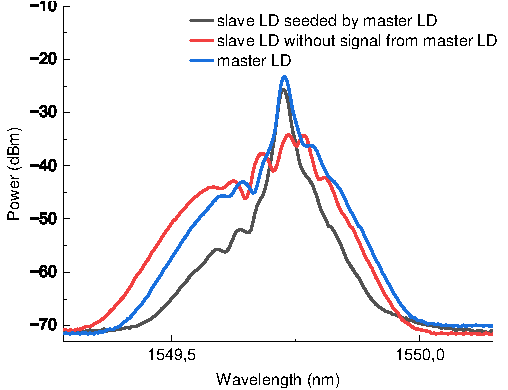
\includegraphics[width=\linewidth]{spectra}
	\caption{Спектры лазерных диодов ведущего, ведомого и источника излучения для КРК}
	\label{fig:QKD_source_spectra}
\end{figure}

\begin{figure}
	\centering
	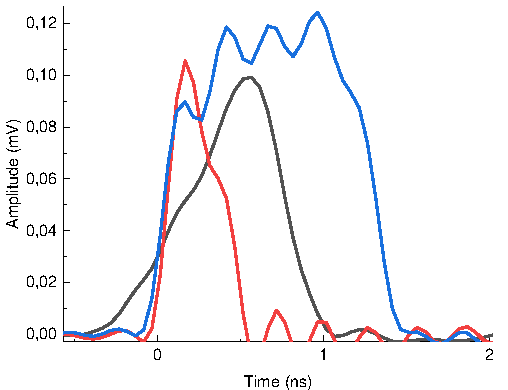
\includegraphics[width=\linewidth]{envelope}
	\caption{Формы импульсов лазеров мастера, слейва и источника излучения КРК}
	\label{fig:QKD_source_pulse}
\end{figure}
%\caption{Spectral characteristics~(a) and pulse envelope~(b) of the master, slave LDs, and adjusted QKD source.}
%\label{fig:QKD_source}

Согласование спектральных характеристик ведущего и ведомого лазеров достигается путем температурной подстройки ЛД с помощью встроенных термоэлектрических элементов. Фактическая частота отстройки, определяемая как разница между пиковыми частотами ведущего и свободно работающего ведомого, составляет менее 6 ГГц. На рисунках \ref{fig:QKD_source_spectra} и \ref{fig:QKD_source_pulse} показаны спектральные характеристики и огибающую импульса ведущего ЛД, свободно работающего ведомого ЛД (без сигнала от ведущего ЛД) и всего источника света (ведомый ЛД, засеянный ведущим ЛД) после настройки. 

Максимальная средняя мощность ведущего лазера на входе в ведомый ЛД составляет 11 мкВт. Чтобы избежать изменения спектральных характеристик при изменении мощности ведущего лазера, она изменяется с помощью микроэлектромеханического переменного оптического аттенюатора VOA (V1550PA, Thorlabs). Управляющее напряжение VOA от 0 до 5 В контролирует затухание, которое может быть увеличено до 25 дБ с помощью напряжения. 

\subsection{Экспериментальная установка}

Наша экспериментальная установка моделирует сценарий, в котором Ева атакует источник QKD из квантового канала. Из-за наличия волоконно-оптического циркулятора в схеме источника Алисы, свет злоумышленника может воздействовать только на ведомый лазер; типичная конструкция волоконно-оптического циркулятора не позволяет свету передаваться от порта 3 циркулятора к порту 1.

В качестве начального лазера злоумышленника мы использовали лазерный диод с распределенной обратной связью (Gooch and Housego AA1406), усиленный волоконным усилителем на основе легированного эрбием и иттербием волокна (EDFA, заказной блок QGLex)\cite{huang2020}. Он работает в непрерывной генерации на рабочей длине волны в диапазоне от 1548.6 до 1550.6 нм. Применяемая в экспериментах мощность составляет около 500 мВт, поскольку дальнейшее увеличение мощности приводит к изменению вносимых потерь и изоляции циркулятора Алисы PMCIR1. Установка Евы также оснащена делителем луча 99:1 и мониторным измерителем оптической мощности, позволяющим измерять мощность Eve в режиме онлайн. Механический регулятор поляризации установлен для достижения минимальных потерь для света злоумышленника в установке. Свет злоумышленника поступает в источник Алисы через сохраняющий поляризацию волоконно-оптический циркулятор PMCIR2 (PMCIR-3-A-1550-900-5-08-FA, Optel). Далее, прежде чем попасть на целевой ведомый лазер, он проходит в обратном направлении циркулятора Алисы PMCIR1, что обеспечивает изоляцию для света злоумышленника примерно в 46-51 дБ . В результате зондирующая мощность атакующего лазера уменьшается из-за этих потерь и достигающая ведомого лазера Алисы, составляет около 1.8 мкВт.

Конфигурация измерений позволяет контролировать среднюю мощность, спектральные, амплитудно-временные характеристики импульсов и интерференцию следующих друг за другом импульсов. Средняя мощность измеряется с помощью оптического измерителя мощности OPM (S154C, Thorlabs). Выходные спектры измеряются оптическим анализатором спектра OSA (AQ6370D, Yokogawa) со спектральным разрешением 0.02 нм. Амплитуда, длительность импульсов, их стабильность и интерференционные сигналы измеряются осциллографами OSC1 и OSC2 (735Zi, Lecroy, полоса пропускания 3.5 ГГц) и p-i-n фотодиодами (PDI35-10G, Thorlabs) с полосой пропускания 10 ГГц. Для анализа статистических распределений амплитуды и длительности оптических импульсов для каждого измерения накапливается 30 тыс. выборок и строится стандартное отклонение. Затем из средних значений амплитуды и длительности и их стандартных отклонений рассчитываются энергия импульса и его стабильность соответственно.
\begin{figure}
	\centering
	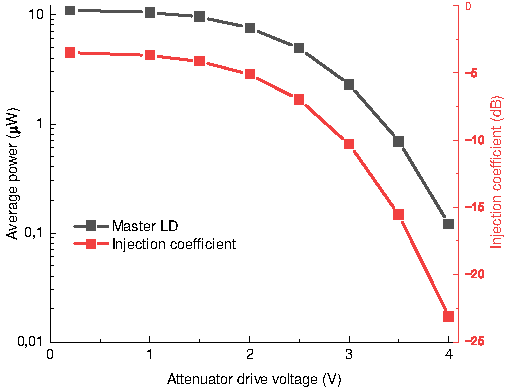
\includegraphics[width=\linewidth]{images/master_power.pdf}
	\caption{Зависимость мощности ведущего лазера (черный) и коэффициента инжекции(красный) от напряжения на аттенюаторе.}
	\label{fig:master_power}
\end{figure}

\begin{figure}
	\centering
	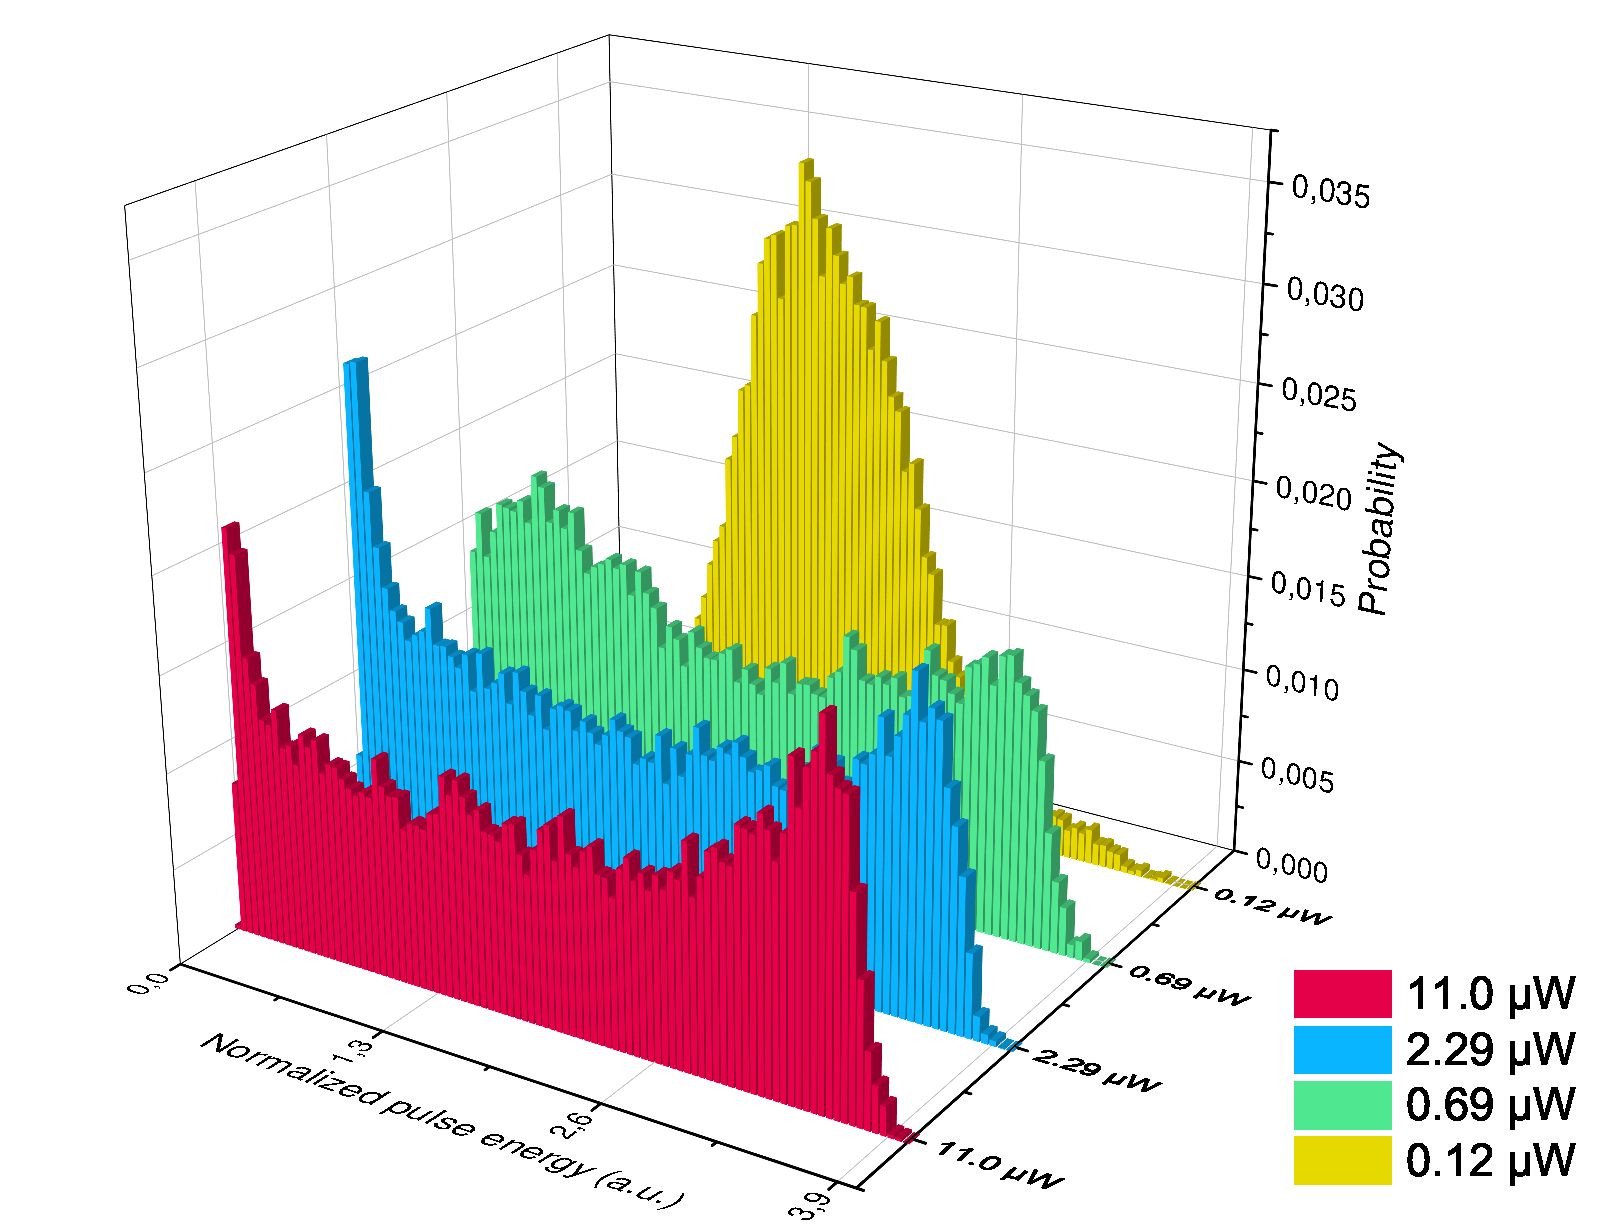
\includegraphics[width=\linewidth]{images/hist_initial.pdf}
	\caption{Функции плотности вероятности интерференции импульсов источника КРК под действием различной мощности лазера-ведущего}
	\label{fig:QKD_PDF}
\end{figure}

\begin{figure}
	\centering
	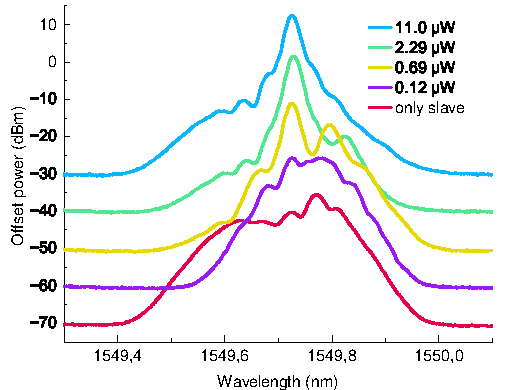
\includegraphics[width=\linewidth]{images/spectra_att.pdf}
	\caption{Спектры излучения лазера-ведомого под действием переменных мощностей лазера-ведущего}
	\label{fig:QKD_spectr}
\end{figure}


\begin{figure}
	\centering
	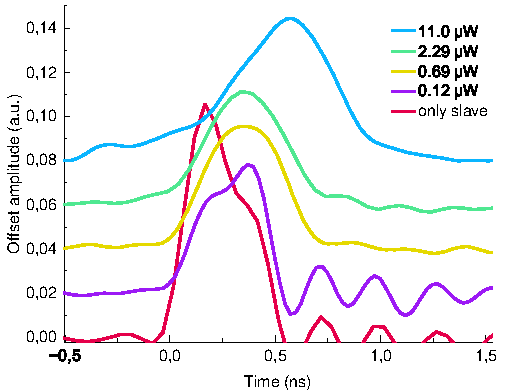
\includegraphics[width=\linewidth]{images/envelope_att.pdf}
	\caption{Формы импульсов лазера-ведомого под действием различных мощностей лазера-ведущего}
	\label{fig:QKD_att}
\end{figure}
%\caption{Характеристики источника QKD в зависимости от напряжения на аттенюаторе: средняя мощность ведущего волокна на входе ведомого волокна (PMCIR1, порт~2) и коэффициент инжекции (a), функция плотности вероятности сигнала помехи (b), выходные спектры (c) и огибающая импульса (d).}


В наших экспериментах мы анализируем качество импульсов, основываясь на форме функции плотности вероятности интерференционного сигнала, как это описано в \cref{sec:theory}. Чтобы обеспечить интерференцию между следующими друг за другом импульсами, мы реализуем полностью волоконный интерферометр Майкельсона на зеркалах Фарадея и с линией задержки длиной около 10 метров. Затем, 20 тысяч измерений площади интерференционного сигнала накапливаются в фиксированном временном интервале (синхронизированном с электрическими импульсами ЛД) для построения гистограммы с помощью встроенного осциллографа.

Во-первых, мы полностью охарактеризовали источник КРК для различных мощностей ведущего ЛД и экспериментально определили границы мощности ведущего ЛД, необходимые для стабильной оптической инжекции. Далее мы провели серию экспериментов по внешней лазерной атаке на Алису и получили зависимости всех характеристик источника лазерного излучения для КРК от средней мощности ведущего ЛД. И, наконец, мы исследовали выходные спектры КРК под воздействием внешнего излучения с различной рабочей длиной волны.
\section{Результаты экспериментов}\label{ch:ch5/sect4}
\label{sec:results}

\subsection{Характеристики источника КРК}

%\Cref{fig:QKD_att} иллюстрирует характеристики источника КРК в зависимости от напряжения управления аттенюатором.

Средняя мощность ведущего ЛД на втором порту PMCIR1 изменяется от 11 до 0.12 мкВт при увеличении напряжения VOA до 4 вольт. Рисунок \ref{fig:injection} демонстрирует эту зависимость и соответствующий расчетный коэффициент инжекции без учета потерь на сопряжении полупроводникового материала с оптическим волокном внутри ведомого лазера (в зависимости от внутренней конструкции ЛД, он может находиться в диапазоне от 1 до 10 дБ). 

Чтобы определить диапазон, в котором ведомый ЛД синхронизируется с излучением ведущего, мы измерили и проанализировали функцию плотности распределения интерференции следующих друг за другом импульсов, спектральные и время-амплитудные характеристики выходных импульсов для каждой мощности ведущего ЛД, построенные на рисунке \ref{fig:master_power}. ФПВ, измеренные для различных мощностей ведущего ЛД на рисунке~\ref{fig:QKD_PDF}, показывают, что синхронизация происходит, когда мощность ведущего ЛД находится в диапазоне от 2.29 до 11 мкВт. Форма ФПВ имеет два пика, соответствующих идеальной конструктивной и деструктивной интерференции. При мощности основного ЛД 0.69 мкВт видность интерференции ухудшается. И, наконец, при минимальной мощности ведущего 0.12 мкВт, ФПВ имеет только один высокий пик в центре. Это означает, что ведомый не имеет оптической синхронизации с ведущим. Без синхронизации временной джиттер импульсов увеличивается, что приводит к увеличению вероятности отсутствия помех.

Из спектров на рисунке \ref{fig:QKD_spectr} и измерений огибающей импульсов на рисунке \ref{fig:QKD_att} также видно, что ведомый ЛД не синхронизируется с излучением ведущего на 0.12 мкВт. В этом случае длина волны выходного сигнала отличается от длины волны ведущего, а также форма выходного импульса далека от идеальной колоколообразной формы, на нее влияют релаксационные осцилляции. В ``граничном'' состоянии при мощности ведущего излучения 0.69 мкВт релаксационные колебания в форме импульса отсутствуют, в то же время его спектр имеет второй интенсивный пик, по частоте отличающийся от частоты ведущего ЛД.

\subsection{Длина волны источника равна длине волны источника}

Как описано в \cref{sec:experiment}, в эксперименте злоумышленником излучается постоянная мощность излучение, в то время как варьируется мощность ведущего лазера. На рисунке~\ref{fig:average_power} демонстрирует зависимость средней мощности источника КРК от мощности ведущего ЛД для двух случаев: в присутствии света Евы и без него. Для оценки средней оптической мощности атакуемого источника КРК мы сначала измеряем общую среднюю мощность, а затем вычитаем отраженную мощность Евы, измеренную при выключенном источнике КРК. Было обнаружено увеличение средней выходной мощности на 6-11\%. Как видно из приведенного графика, монотонной зависимости увеличения мощности от мощности ведущего ЛД не наблюдается. Увеличение мощности значительно варьируется при малом сигнале ведущего устройства и становится постоянным около $8~\%$, когда мощность ведущего устройства составляет от 7.57 до 11 мкВт.
\begin{figure}
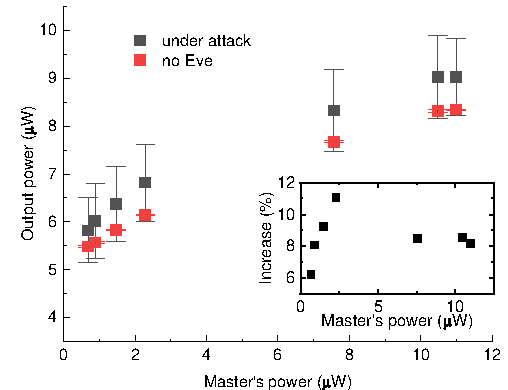
\includegraphics[width=\linewidth]{average_power}
\caption{Средняя выходная мощность источника КРК без Евы и в присутствии атаки с лазерным засевом.}
\label{fig:average_power}
\end{figure}
Однако более важным является вопрос о том, насколько сильно изменяется энергия импульса. Чтобы ответить на этот вопрос, сначала измерялась средняя амплитуда и длительность импульса, а также их стандартное отклонение, рассчитанное на основе выборки размером 30 тысяч. Рисунок~\ref{fig:area} показывает измеренные амплитуду и длительность, а также рассчитанную нормализованную энергию импульса с атакой и без нее. Из рисунков \ref{fig:amplitude} и \ref{fig:duration} видно, что средняя амплитуда импульса увеличивается при атаке, в то время как длительность импульса почти такая же, как и без атаки. Отклонения обеих измеренных величин увеличиваются при атаке. Энергия импульса рассчитывается как умножение измеренной средней амплитуды на среднюю длительность, а стандартное отклонение энергии импульса (СО) - как квадратный корень из суммы квадратов СО измеренных амплитуды и длительности. (Следует отметить, что примененный метод расчета корректен в случае наших экспериментальных данных, поскольку все измеренные формы импульсов имеют однопиковую форму, близкую к колоколообразной, в то время как в общем случае, когда импульсы имеют сложную форму, энергия может перераспределяться между пиками, и, таким образом, площадь импульса должна быть получена из прямых измерений, а не из отдельных измерений амплитуды и длительности импульса). \Cref{fig:area} показывает энергию импульса с атакой и без атаки, нормированную на энергию без атаки при каждой мощности ведущего ЛД. Вставленный график демонстрирует стандартное отклонение энергии импульса для обоих случаев. Изменение энергии импульса при атаке не показывает зависимости от мощности ведущего ЛД, она распределяется хаотично. Максимальное увеличение средней энергии импульса составляет $2,8\%$, когда мощность ведущего ЛД равна 7.57 мкВт. В то же время, колебания энергии импульса увеличиваются во всех исследованных случаях. Стандартное отклонение стало выше примерно на 3\% при атаке по сравнению с результатами без атаки.

В рамках работы также проведена оценка временного джиттера в присутствии и без атаки. Он определяется как стандартное отклонение измерения периода при 30 тыс. отсчетов. Оно составляет 125-128 пс без света Евы и почти такое же 126-130 пс в присутствии атаки. 

\begin{figure}%{0.3\linewidth}
	\centering
	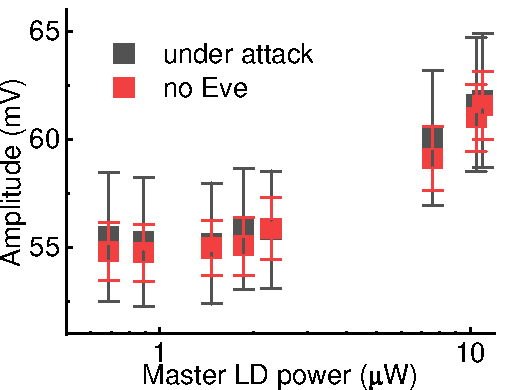
\includegraphics[width=\linewidth]{images/amplitude_change.pdf}
	\caption{Изменение средней амплитуды импульсов. Черным цветом обозначены амплитуды импульсов под действием атаки, а красным без нее.}
	\label{fig:amplitude}
\end{figure}


\begin{figure}%{0.3\linewidth}
	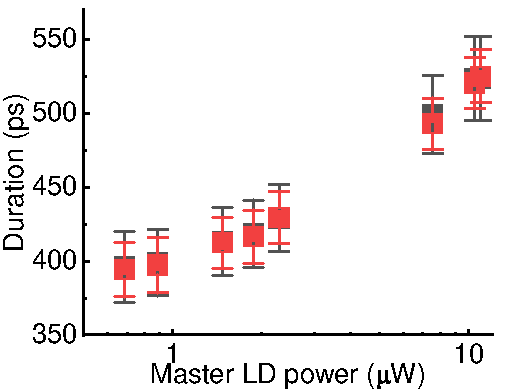
\includegraphics[width=\linewidth]{images/duration_change.pdf}
	\caption{Изменение средней длительности импульсов. Черным цветом обозначены длительности импульсов под действием атаки, а красным без нее.}
	\label{fig:duration}
\end{figure}


\begin{figure}%{0.3\linewidth}
	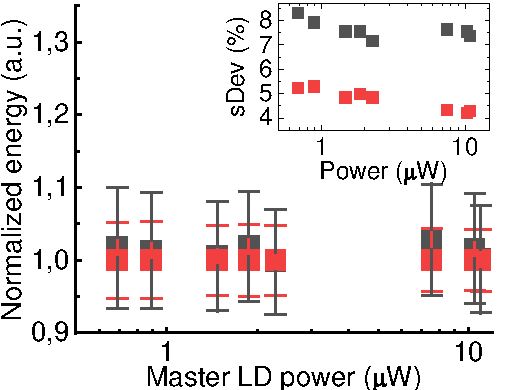
\includegraphics[width=\linewidth]{images/area_under_attack.pdf}
	\caption{Изменение средней площади импульсов. Черным цветом обозначены площади импульсов под действием атаки, а красным без нее.}
	\label{fig:area}
\end{figure}
%\caption{Характеристики импульсов с атакой и без: (a)~амплитуда, (b)~длительность и (c)~вычисленная нормализованная энергия импульса (стандартное отклонение указано на вставленном графике).}


\begin{figure}
	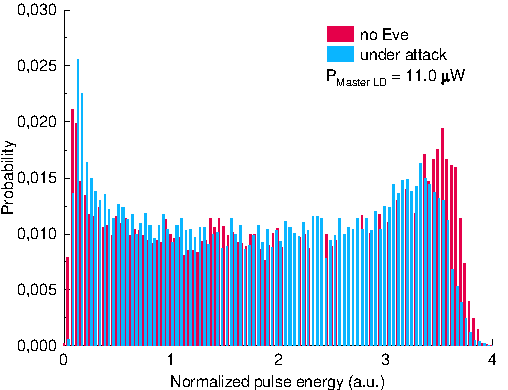
\includegraphics[width=\linewidth]{images/hist_attack_11.pdf}
	\caption{Функция плотности вероятности интерференции при мощности лазера-ведущего 11 мкВт. Красным обозначена ФПВ без атаки, синим цветом обозначена ФПВ под действием атаки.}
	\label{fig:histogram_max}
\end{figure}


\begin{figure}
	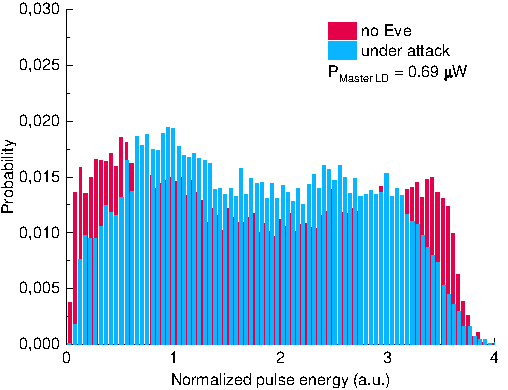
\includegraphics[width=\linewidth]{images/hist_attack_01.pdf}
	\caption{Функция плотности вероятности интерференции при мощности лазера-ведущего 0.69 мкВт. Красным обозначена ФПВ без атаки, синим цветом обозначена ФПВ под действием атаки.}
	\label{fig:histogram_min}
\end{figure}
%\caption{Функция плотности вероятности нормированного сигнала помех с атакой и без нее: (a)~ мощность ведущего LD составляет 11 мкВт; (b)~ мощность ведущего LD составляет 0,69 мкВт.}


Предполагается, что разница между увеличением средней мощности и энергии импульса означает, что наибольший вклад в увеличение средней мощности вносит усиление излучения Евы в ведомом лазере, а не изменение выходных импульсов. Слабое увеличение энергии импульса и стабильное повышение его стабильности обусловлены слабыми изменениями числа электронов в валентной зоне, вызванными стимулированным поглощением инжектированного света Евы. 

В наших экспериментах мы также количественно оценили влияние инжектированного света на статистику интерференции. \Cref{fig:histogram_max} и \Cref{fig:histogram_min} позволяет сравнить функции плотности вероятности интерференционного сигнала со светом Евы и без него для двух граничных случаев - когда ведущий лазер принимает максимальное и минимальное значения для обеспечения синхронизации. В обоих случаях мы наблюдаем изменения в ФПВ из-за атаки внешним излучением.

Чтобы количественно оценить влияние света Евы на интерференцию, видимость интерференции оценивается по \cref{eq:visibility}, где ожидаемые интенсивности конструктивной и деструктивной интерференции берутся по пиковым значениям вероятности экспериментальных ФПВ. Видность уменьшается примерно с 86.4 до 80.1 , когда мощность ведущего устройства принимает максимальное значение в 11 мкВт, примерно с 71.5 до 52.5, когда мощность ведущего устройства составляет 0.69 мкВт . Таким образом, влияние света злоумышленника на интерференционный сигнал усиливается с уменьшением соотношения мощностей лазера-ведущего и лазера Евы. Возможно, что этот эффект вызван смешением усиленного света Евы с интерферирующими импульсами Алисы и, как было показано в начале текста, увеличением колебаний энергии импульсов, а не фазовой перестройкой между светом ведущего и Евы при его усилении в ведомом ЛД.
\subsection{Атака в зависимости от длины волны}.
В этом разделе исследуется влияние лазера Евы, работающего на разных длинах волн, на выходной спектр источника КРК. Длина волны атакующего лазера изменялась в зависимости от температуры диода его затравочного лазера, а мощность инжектируемого света Евы была одинаковой во всех измерениях.

\begin{figure}
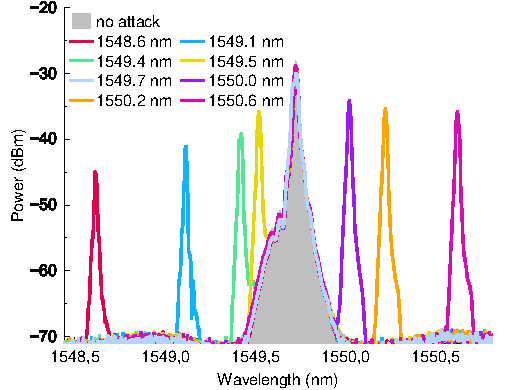
\includegraphics[width=\linewidth]{WL_Eve}
\caption{Спектры выходного сигнала источника QKD для разных длин волн лазера Евы. (Спектры отраженного излучения Евы исключены из измеренных выходных спектров)}.
\label{fig:WL_Eve}
\end{figure}

\Cref{fig:WL_Eve} показывает выходные спектры для различных длин волн затравочного лазера. Спектры атакуемого КРК источника и отраженного излучения Евы с выключенным QKD-источником измеряются отдельно. Далее, чтобы оценить, усиливает ли ведомый лазер излучение Евы или нет, отраженные спектры вычитаются из спектров атакуемого источника QKD.

Отметим, что реализованная процедура измерения не является точной для получения коэффициентов усиления, более того, спектральное разрешение в 0.02 нм дает лишь грубую оценку спектральных характеристик при определении характеристик DFB-лазеров. Однако этого достаточно, чтобы показать, что излучение Евы усиливается ведомым лазером в широком спектральном диапазоне.

\section{Выводы по главе}\label{ch:ch5/sect5}
В рамках данной главы впервые рассматривалась атака "засевом" лазерным излучением источника на основе оптической инжекции для систем квантового распределения ключей. В результате работы было оценено влияние атаки злоумышленника с помощью лазера мощностью в 500 мВт. 
Эта атака приводит к увеличению средней мощности излучения до $11\%$, увеличивает энергию импульсов на $2.8\%$ и стандартное отклонение их амплитуды на 3\%. При этом длительность импульсов не изменяется.
Также был рассмотрен вопрос усиления других длин волн излучения злоумышленника. Источник излучения, построенный на основе оптической инжекции, является устойчивым к атаке лазерным "засевом" благодаря наличию оптического циркулятора и дополнительного внешнего излучения от лазера-ведущего.
В результате чего злоумышленнику необходимо как пройти изоляцию этого циркулятора, так и превзойти лазер-ведущий, чтобы осуществить атаку. Это возможно только с помощью высокомощного излучения, которое смогут обнаружить легитимные пользователи.
\newline Влияние атаки лазерным засевом на источник излучения на основе оптической фазовой синхронизации может быть предотвращено достаточным количеством изоляции, а также оптическими предохранителями для защиты от мощного излучения.